\documentclass[11pt]{amsart}
\usepackage{geometry}                % See geometry.pdf to learn the layout options. There are lots.
\geometry{letterpaper}                   % ... or a4paper or a5paper or ... 
%\geometry{landscape}                % Activate for for rotated page geometry
%\usepackage[parfill]{parskip}    % Activate to begin paragraphs with an empty line rather than an indent
\usepackage{graphicx}
\usepackage{amssymb}
\usepackage{epstopdf}
\usepackage{sidecap}
\DeclareGraphicsRule{.tif}{png}{.png}{`convert #1 `dirname #1`/`basename #1 .tif`.png}

\title{Ifstool, digital support for Image Analysis Research}
\author{The Author}
%\date{}                                           % Activate to display a given date or no date

\begin{document}
\maketitle
%\section{}
%\subsection{}
Ifstool is a GUI which supports the Image Analysis researcher. It supports images of any size\footnote{Until the process runs out of memory}, any number of dimensions\footnote{Also limited by memory capacity}, and a wide variety of formats. 

The program runs on Linux, Mac OSX, and Windows 7, 8 and 10. Files are interchangeable between platforms. Conversion from 3d images to movies (xxx) is also included. The program can do  Fourier analysis, and filtering.

Finally, the program can run an external script, writing an image out, running the script, and reading the script back in, thus providing general image analysis capability.

\section{Input File Formats}
Internally, Ifstool uses IFS (Image File System). All images are converted into ifs. Ifs supports any computer data type, including complex. Ifstool can read images in any of the following formats

\begin{itemize}
\item Portable Network Graphics (PNG, png)
\item Joint Photographics Experts Group (JPG, jpg, jpeg)
\item Tagged Image File Format (TIFF, tif, tiff)
\item Image File Format) (IFS, ifs)
\item Graphics Interchange Format (GIF)
\item Bitmap File Format (bmp)
\end{itemize}

\section{Organization of Data}
If the user has bound the Ifstool to a class of files (e.g. png), then one may simply double click  a file and the application will load the file.
Or, the user may choose to press the open  button. A file select window will open, and the user may select the desired file.

Ifstool maintains eight image buffers, numbered 0-7, as illustrated in Figure \ref{fig:InputSelect}. Any of the 8 image buffers may be denoted as INPUT1, INPUT2, or OUTPUT. The Open operation will load the target file into the image buffered selected as INPUT1.
\begin{SCfigure}
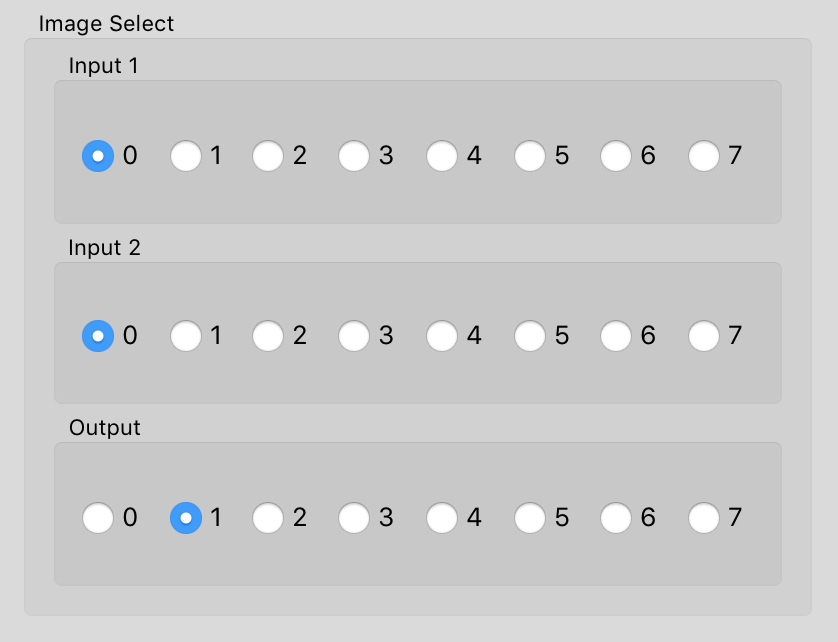
\includegraphics[width=3in]{InputSelect.png}
\caption{Any of eight different images may be used as input or output.}
\label{fig:InputSelect}
\end{SCfigure}

The internal buffer will be of type ``float'' or ``complex float'', and have the same number of dimensions as the selected input image. If the image is color (as is default for png), it will be three dimensions and have 3 frames. An image may also be three dimensions and not be color. For example ``movie loops'' may allow the user to play a sequence of images.



\subsection{Viewing Complex Images}
If the image selected as OUTPUT is complex, the user should select it as INPUT1, and use the COMPLEX pulldown. Operations are listed below:
\begin{description}
\item[Magnitude] will compute the magnitude of the INPUT1 buffer and return it in the selected output buffer. This operation requires complex input.
\item[Phase] will compute the phase of the INPUT1 buffer and return it in the selected output buffer. This operation requires complex input.
\item[Real] will extract the real part  of the INPUT1 buffer and return it in the selected output buffer. This operation requires complex input.
\item[Imaginary] will extract the imaginary part  of the INPUT1 buffer and return it in the selected output buffer. This operation requires complex input.
\end{description}
%\section{File Operations}
\section{File Operations}
Most file operations may be accessed by either the file pulldown, or across the top of the main window as illustrated below:

%
\includegraphics[width=3in]{filepulldown.png}

\includegraphics[width=4in]{filepulldown.png}
%\section{Unary (one input) Operations}
\subsection{Open}
This operation will open a file selection window, allowing the user to choose any data type of image file listed above. It will be read into whichever buffer is marked INPUT1.
\section{Reopen}

\includegraphics[width=3in]{ReOpen.png}

Once a file has been read, Ifstool saves the name of that file in two places, in the program and on the disk.  Clicking Reopen will read the file as stored in the archive program, and if that string is empty, it open the file as specified in the file list on disk. Thus, even the first time the program is loaded, using Reopen will load an image (unless, of course, the program has never previously been run). 

\section{SaveAs}
Save the buffer selected as OUTPUT to any data type or format. Including png, jpg, and ifs. If the output data type is ifs, a popup will ask the user to specify the data type.  At this time, only the ifs data type is implemented.
\section{Copy}
Copies a selected output buffer.

\section{Paste}
Pastes a copied buffer to currently selected output buffer.
\section{Viewing an Image}
When the {\em view} button is pushed, the image selected as OUTPUT will be displayed into a new window, called {\em the viewing window} here. 
If the image selected as OUTPUT is 2-D or color, the {\em View} button will display that image. Complex color is not supported.

There are additional functions available on the viewing window. 
These include:
\begin{description}
\item[Choice of Frame Number] A color image may be considered as composed of three images, red, green, and blue. Usually, the user seeks to view the three together as a single color image, and if the color check box is checked, this is the model.  However, the user may choose to view each frame independently as a single gray scale image. That view mode is used if the color check box is unchecked. 

Images consisting of more than three frames can also be viewed by unsetting the color check box and clicking the frame select button.
\item[Color Model] The appearance of an image may be modified by  adding or  subtracting yellow or blue to increase the ``warmth'' or ``coolness'' of the image. These modifications are only made in the display buffer, and modifying them does not affect the master images, (those stored in buffers 0-7).
\item [Color Enhancement]
The appearance of an image may also be modified by  adjusting the degree of red, green, or blue in  f the image. These modifications are only made in the display buffer, and modifying them does not affect the master images, (those stored in buffers 0-7).

\item[Zoom] Using the zoom slider makes the viewed image larger or smaller, but does not affect the master images, (those stored in buffers 0-7).
\item[Window and Level]
Window and level are parameters used to enhance or reduce contrast. The terms {\em window} and {\em level} are most meaningful if one considers an image in which the brightness values range between, say, 0 and 1023, but use a display which can only display brightnesses between 0 and 255. The {\em window} defines the brightness rang which is mapped (linearly) to lie between 0 and 255. For example, that might be brightnesses between 0 and 50. The {\em level} defines where the window lies. For example, a window with wi
\end{description}

\section{Unary (one input) Operations}
The input image to all the unary operations is the one selected as INPUT1. The output will be the one selected as OUTPUT.
\begin{description}
\item[$\frac{\partial f}{\partial x}$] Computes a fast estimate of the  derivative of brightness with respect to x (the column direction).
\item[$\frac{\partial f}{\partial y}$] Computes a fast estimate of the  derivative of brightness with respect to y (the row direction).
\item[$\frac{\partial^2 f}{\partial x^2}$] Computes a fast estimate of the  second derivative of brightness with respect to x (the column direction).
\item[$\frac{\partial^2 f}{\partial y^2}$]Computes a fast estimate of the  second derivative of brightness with respect to y (the row direction).
\item[$\frac{\partial^2 f}{\partial y\partial y}$] Computes a fast estimate of the  second derivative of brightness with respect to x and y (the cross term).
\item[Exponential] Computes $\exp (f(x,y)$ at each point in the image.
\item[Inverse]
\item[Laplacian] Computes $\frac{\partial^2 f}{\partial x^2} + \frac{\partial^2 f}{\partial y^2}$ at each point in the image.
\item[NatLog] Computes $\ln f(x,y)$ at each point.
\item[HistEq] Histogram equalization finds the image whose histogram is as close to flat as possible.
\item[PseudoColor] Given a 2D grayscale image in INPUT1, OUTPUT will be a color image where the brightness of each pixel has been remapped to a color. The user must specify how the mapping occurs using a ``colormap.'' Possible maps are
\begin{itemize}
\item 0: gray scale
\item 1: inverse gray scale
\item 2: Bronson
\item 3: Hot metal
\item 4: Heated Spectrum
\item 5: Log
\item 6: Random
\end{itemize}
The Random map is surprisingly useful when evaluating noise removal algorithms. Because the colors are assigned randomly, if two adjacent points are identical in brightness, they will be displayed as the same color. Therefore large areas of constant color suggest a very smooth image. 

{\em The output from colormap is a 3D, 3 frame, unsigned char image. That image may be saved using saveAs.}

\end{description}

\section{Binary Operations}
At this time, the only operations with two inputs are add, subtract, multiply, and divide. They work correctly with both float and complex data types.
\section{Frequency Domain Operations}
All frequency domain operations are accessed via the COMPLEX pulldown.
\begin{description}
\item[fft] will compute the Fourier transform of INPUT1. Internally, this uses the complex two-dimensional fast Fourier transform. Images having dimension which are not a power of 2 will be padded. If the input is real, it will be copied into a complex image first. If the input is three-dimensional (a movie) or color, the fft is only applied to the first frame.

Note that the origin of the FFT will be at 0,0, the upper left of the image. Fourier transforms are often displayed with the origin in the center of the image, showing negative frequencies as positive. If the user is expecting this, the results may be surprising. In particular, instead of the DC term being in the center of the image, it will be at the upper left.
\item[ifft] will compute the inverse Fourier transform of INPUT1. Internally, this uses the complex two-dimensional fast Fourier transform. Images having dimension which are not a power of 2 will be padded. The input image must be complex. 
\item[Complex Magnitude] Constructs a float image from a complex image by calculating the magnitude of the complex number.
\item[Complex Phase] Constructs a float image from a complex image by calculating the phase of the complex number.
\item[Real] Constructs a float image from a complex image by extracting the real part of the complex number.
\item[Imaginary] Constructs a float image from a complex image by extracting the imaginary of the complex number.
\end{description}
\section{Window and Level}
The Window and Level operations allow the user to modify the contrast and brightness in a convenient way, even if the input image has brightnesses which range outside the usual 0 to 255.

\begin{description}
\item[Window] is the brightness range which will be mapped to 0-255 on the display. Making this larger or smaller is equivalent to making the contrast lower or higher.
\item[Level] is the location, in brightness, of the center of the window. 
\end{description}
 Note that if a pixel brightness is below level-window/2 it will be mapped to zero, and if it is above level+window/2, it will be mapped to 255. So the window-level operation has the same result to setting an upper threshold and a lower threshold, and scaling the levels in between to 0-255.
\end{document}  